\documentclass[
	%parspace, % Térköz bekezdések közé / Add vertical space between paragraphs
	%noindent, % Bekezdésének első sora ne legyen behúzva / No indentation of first lines in each paragraph
	%nohyp, % Szavak sorvégi elválasztásának tiltása / No hyphenation of words
	%twoside, % Kétoldalas nyomtatás / Double sided format
	%draft, % Gyorsabb fordítás ábrák rajzolása nélkül / Quicker draft compilation without rendering images
	%final, % Teendők elrejtése / Set final to hide todos
]{elteikthesis}[2020/11/23]

% Dolgozat metaadatai
% Document's metadata
\title{Dolgozat címe} % cím / title
\date{2020} % védés éve / year of defense

% Szerző metaadatai
% Author's metadata
\author{Hallgató Hanga}
\degree{programtervező informatikus BSc}

% Témavezető(k) metaadatai
% Superivsor(s)' metadata
\supervisor{Témavezető Tamás} % belső témavezető neve / internal supervisor's name
\affiliation{egyetemi tanársegéd} % belső témavezető beosztása / internal supervisor's affiliation
%\extsupervisor{Külső Kornél} % külső témavezető neve / external supervisor's name
%\extaffiliation{informatikai igazgató} % külső témavezető beosztása / external supervisor's affiliation

% Egyetem metaadatai
% University's metadata
\university{Eötvös Loránd Tudományegyetem} % egyetem neve / university's name
\faculty{Informatikai Kar} % kar neve / faculty's name
\department{Programozáselmélet és Szoftvertechnológiai\\ Tanszék} % tanszék neve / department's name
\city{Budapest} % város / city
\logo{elte_cimer_szines} % logo

% Irodalomjegyzék hozzáadása
% Add bibliography file
\addbibresource{thesis.bib}

% A dolgozat
% The document
\begin{document}

% Nyelv kiválasztása
% Set document language
\documentlang{magyar}
%\documentlang{english}

% Teendők listája (final dokumentumban nincs)
% List of todos (not in the final document)
%\listoftodos[\todolabel]

% Dokumentum beállítások
% Some document settings
% Lábjegyzet folytonos számozása fejezetek között
% Continuous counting of footnotes among chapters
\counterwithout{footnote}{chapter}

% Tartalomjegyzék oldalszámozásának rejtése
% Hide page numbering of ToC
\newcounter{conpageno}
\let\oldtableofcontents\tableofcontents
\renewcommand{\tableofcontents}{
	\pagenumbering{gobble}
	\oldtableofcontents
	\cleardoublepage
	\setcounter{conpageno}{\value{page}}
	\pagenumbering{arabic}
	\setcounter{page}{\value{conpageno}}
}


% Címlap (kötelező)
% Title page (mandatory)
\maketitle
\topicdeclaration

% Tartalomjegyzék (kötelező)
% Table of contents (mandatory)
\tableofcontents
\cleardoublepage

% Tartalom
% Main content
\chapter{Bevezetés} % Introduction
\label{ch:intro}

Lorem ipsum dolor sit amet, consectetur adipiscing elit. In eu egestas mauris. Quisque nisl elit, varius in erat eu, dictum commodo lorem. Sed commodo libero et sem laoreet consectetur. Fusce ligula arcu, vestibulum et sodales vel, venenatis at velit \cite{dahl1972structured}. Aliquam erat volutpat. Proin condimentum accumsan velit id hendrerit. Cras egestas arcu quis felis placerat, ut sodales velit malesuada. Maecenas et turpis eu turpis placerat euismod.\footnote{Maecenas a urna viverra, scelerisque nibh ut, malesuada ex.}

Aliquam suscipit dignissim tempor. Praesent tortor libero, feugiat et tellus porttitor, malesuada eleifend felis. Orci varius natoque penatibus et magnis dis parturient montes, nascetur ridiculus mus \cite{cormen2009algorithms,krasner1988mvc}. Nullam eleifend imperdiet lorem, sit amet imperdiet metus pellentesque vitae. Donec nec ligula urna. Aliquam bibendum tempor diam, sed lacinia eros dapibus id. Donec sed vehicula turpis. Aliquam hendrerit sed nulla vitae convallis. Etiam libero quam, pharetra ac est nec, sodales placerat augue. \citeauthor{dijkstra1979goto} praesent eu consequat purus \cite{dijkstra1979goto}. 

\cleardoublepage

\chapter{Felhasználói dokumentáció} % User guide
\label{ch:user}

\section{Bejelentkezés és nyelvválasztás}
Az oldalra érkezve a kezdőoldalt láthatjuk, ahol egy üdvözlő üzenet fogad minket. Majd lehetőségünk nyílik bejelentkezni a rendszerbe, vagy a rendszer által támogatott lokalizációt tudjuk kiválasztani (\ref{fig:main-page} ábra). \footnote{Erre majd még a bejelentkezés után is lehetőségünk nyílik lásd később,~\hyperref[step:mindenkinek-elerheto-oldal]{\ref{step:mindenkinek-elerheto-oldal}:~``Mindenki számára elérhető oldalak''}}
\begin{figure}[H]
	\centering
	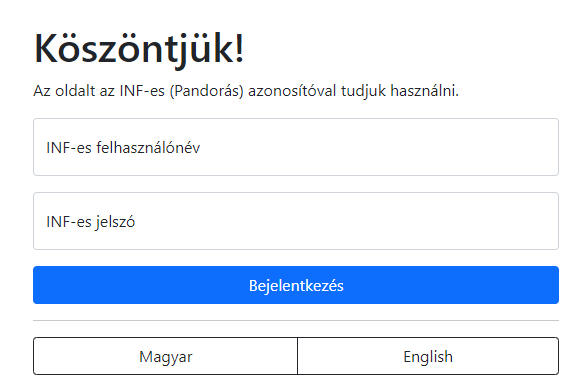
\includegraphics[width=0.6\textwidth]{userguide/main-page}
	\caption{Főoldal}
	\label{fig:main-page}
\end{figure}
\subsection{Bejelentkezés}
A rendszerbe bejelentkezni az INF-es felhasználónkkal tudunk. Ha a bejelentkezés sikertelen volt, azt a rendszer hibaüzenetekkel jelzi a számunkra (\ref{fig:login-error} ábra). 
\begin{figure}[H]
	\centering
	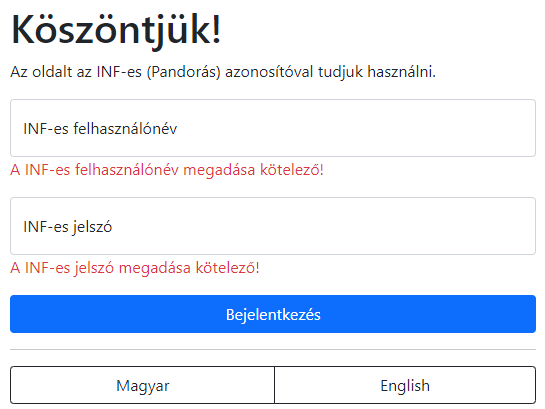
\includegraphics[width=0.6\textwidth]{userguide/login-error}
	\caption{Bejelentkezési hiba}
	\label{fig:login-error}
\end{figure}
Amennyiben a bejelentkezés sikeres volt, a \emph{szerepkörnek} megfelelő kezdőoldalon találjuk magunkat (\ref{fig:logged-in} ábra).
\begin{figure}[H]
	\centering
	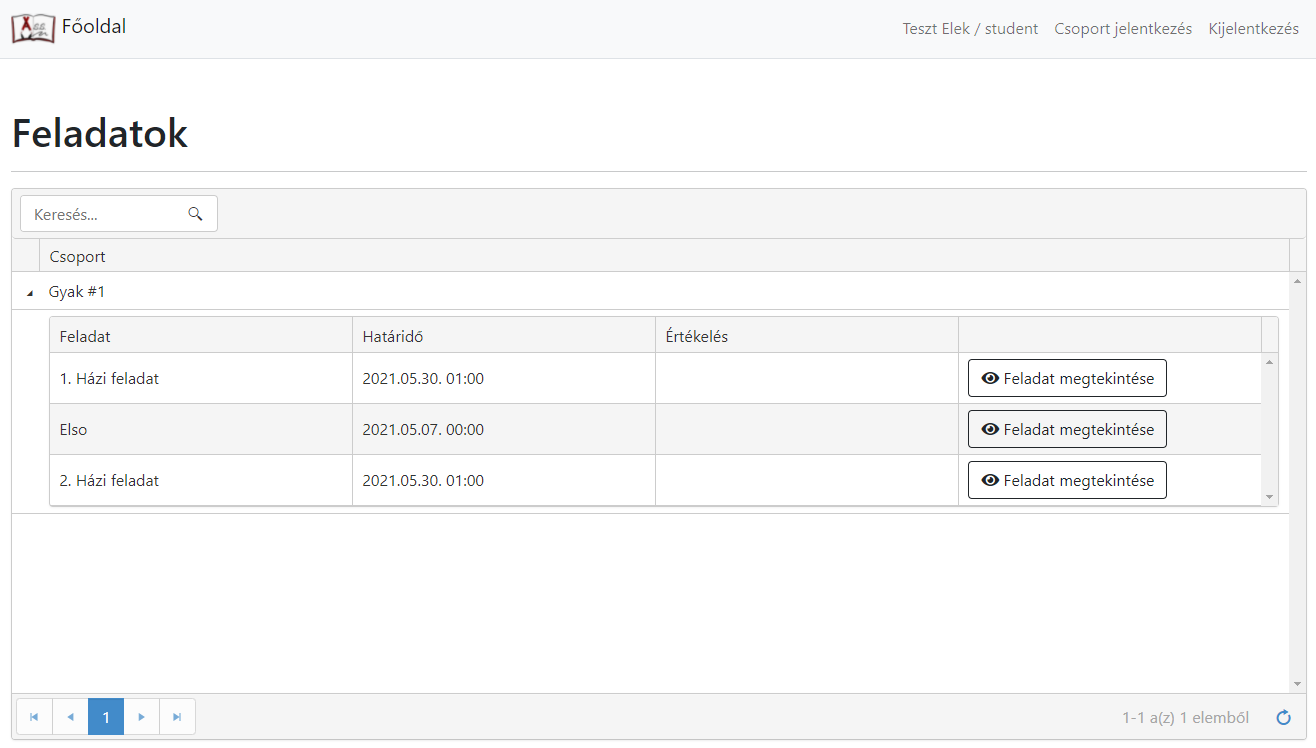
\includegraphics[width=1.0\textwidth]{userguide/logged-in}
	\caption{Sikeres bejelentkezés}
	\label{fig:logged-in}
\end{figure}
\subsection{Nyelvválasztás}
A rendszer kilistázza a támogatott lokalizációkat (jelenleg magyar és angol). Alapértelmezett beállítás a magyar. Ezt felültudjuk írni, ha valamelyik gombra rákattintunk. (\ref{fig:change-lang} ábra)
\begin{figure}[H]
	\centering
	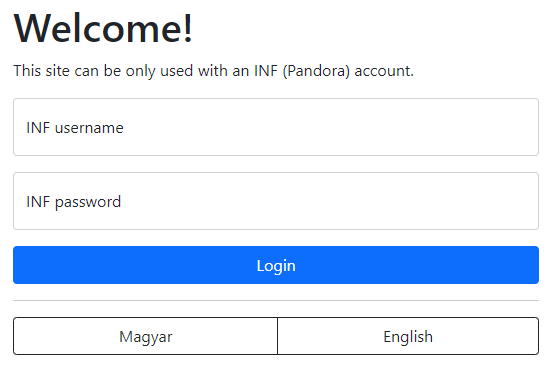
\includegraphics[width=0.6\textwidth]{userguide/change-lang}
	\caption{Nyelvváltás}
	\label{fig:change-lang}
\end{figure}
\section{Szerepkörök}
A felhasználók négy csoportba tartozhatnak:
\begin{compactitem}
    \item \hyperref[step:admin-role]{Rendszergazda}
    \item \hyperref[step:teacher-role]{Tárgyfelelős}
    \item \hyperref[step:instructor-role]{Gyakorlatvezető}
    \item \hyperref[step:student-role]{Hallgató}
\end{compactitem}
Egy felhasználó tartozhat több szerepkörbe. Ha egy felhasználó több szerepkörbe is tartozik, akkor a felület menüsorán megjelenik egy "Szerepkör váltás" lenyitható menü, ahol a felhasználóhoz rendelt szerepköröket találjuk, a kiválasztott linkre kattintva a csoporthoz tartozó kezdőoldalra navigáljuk magunkat. A felhasználóhoz a szerepköröket a felhasználó létrehozásakor is megadhatjuk, valamint a létrehozást követően tudjuk módosítani.
\subsection{Rendszergazda}\label{step:admin-role}
A rendszergazda a következő funkciókat érheti el:
\begin{compactitem}
    \item Tantárgy létrehozása, módosítása, törlése, tárgyi információk megtekintése
    \item Felhasználó létrehozása, módosítása, a felhasználók adatainak a megtekintése
\end{compactitem}
Ha rendszergazdaként jelentkezünk be az alábbi két táblázat fogad minket a kezdőoldalon~(\ref{fig:admin-page} ábra). 
\begin{figure}[H]
	\centering
	\subfigure[Tantárgyak táblázata]{
		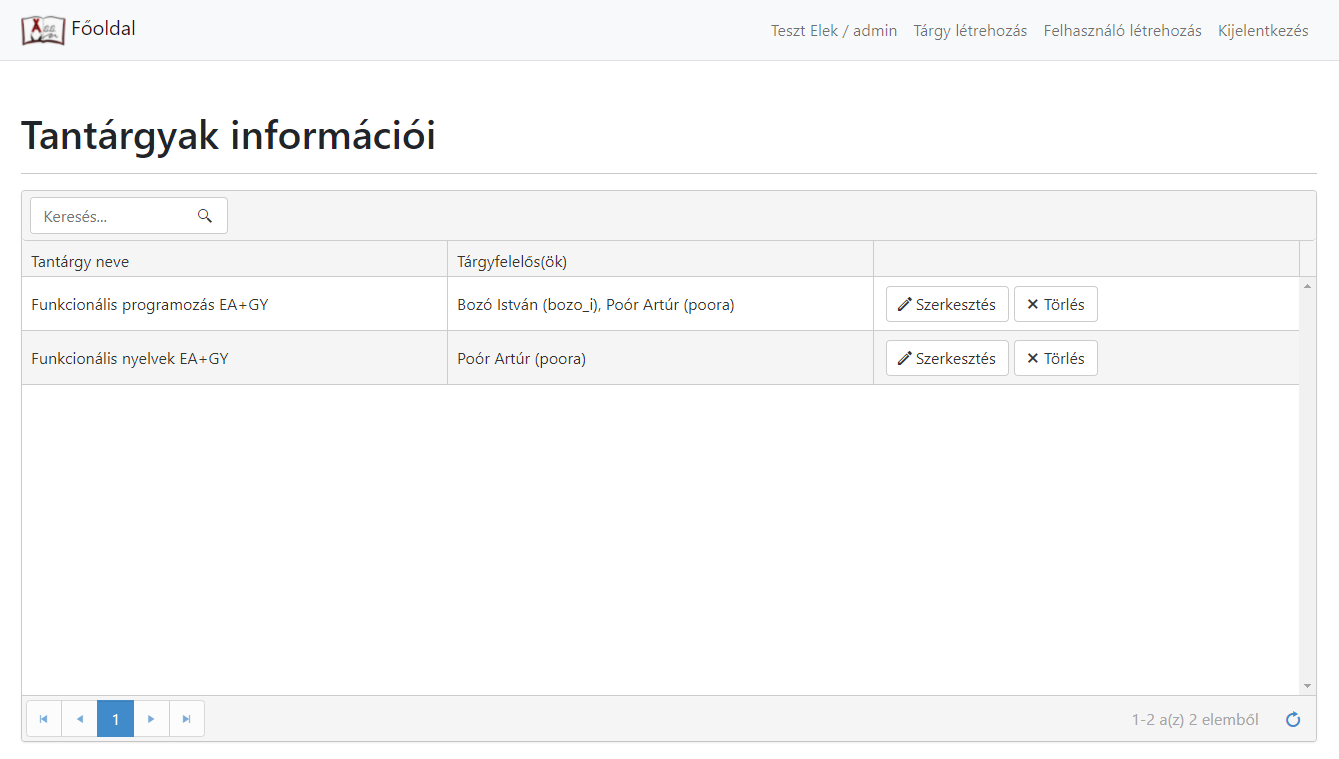
\includegraphics[width=1\linewidth]{userguide/admin-table1}
        \label{subfig:admin-subject-table}}
	\hspace{5pt}
	\subfigure[Felhasználók táblázata]{
		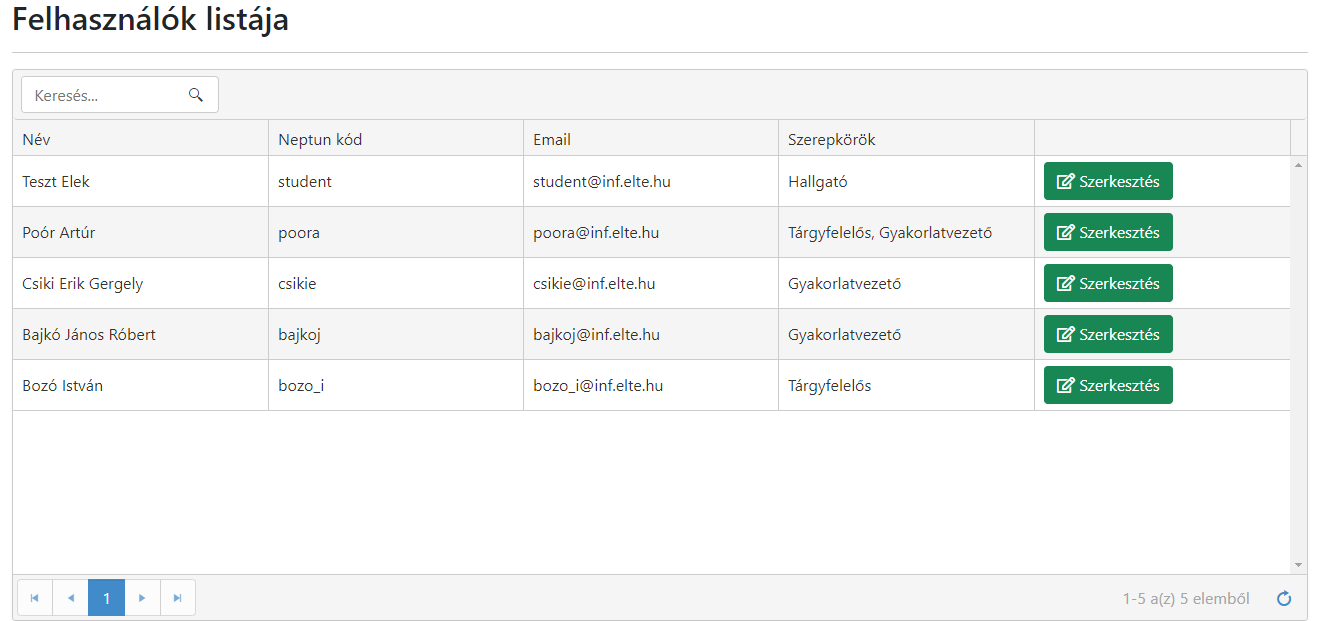
\includegraphics[width=1\linewidth]{userguide/admin-table2}
        \label{subfig:admin-users-table}}
	\caption{Rendszergazdai szerepkör kezdőoldala}
	\label{fig:admin-page}
\end{figure}
Az első táblázatban a rendszerben létrehozott tantárgyak és a hozzájuk tartozó információk olvashatóak le. A táblázatban az egyes tantárgyakhoz tartozó adatok módosíthatóak, illetve az egész tárgyat lehet törölni. A módosítás során validálásra kerül, hogy a módosított név létezik-e már a rendszerben, ha igen, akkor ezt a rendszer jelzi számunkra. A második táblázatban a rendszerben létrehozott felhasználókat és a hozzájuk tartozó információkat láthatjuk. A rendszergazda a felhasználók adatait és szerepköreit tudja módosítani.
\subsubsection{Tantárgy létrehozása}
A ``Tárgy létrehozás'' linkre kattintva az alkalmazás átnavigál minket egy űrlapra, ahol az új tantárgy szükséges adatait tudjuk kitölteni (\ref{subfig:admin-create-subject} ábra). Ha az adatok validálása és feldolgozása sikeres, akkor visszanavigálódunk a kezdőoldalra. Az esetleges validalási hibákat a rendszer jelzi számukra (\ref{subfig:admin-create-subject-error} ábra).
\begin{figure}[H]
	\centering
	\subfigure[Űrlap]{
		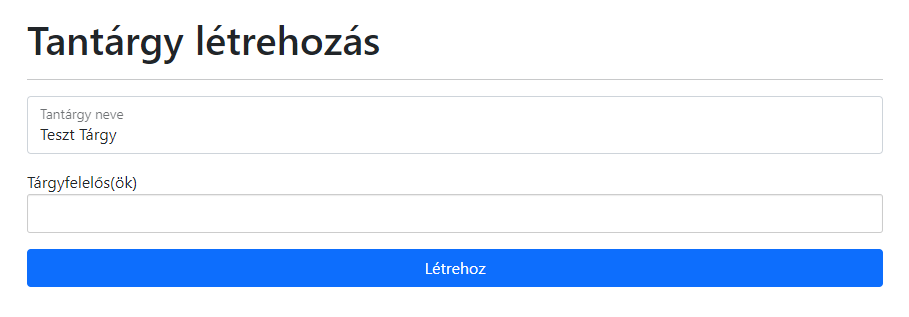
\includegraphics[width=0.8\linewidth]{userguide/admin-create-subject-form}
        \label{subfig:admin-create-subject}}
	\hspace{5pt}
	\subfigure[Adatok validálása]{
		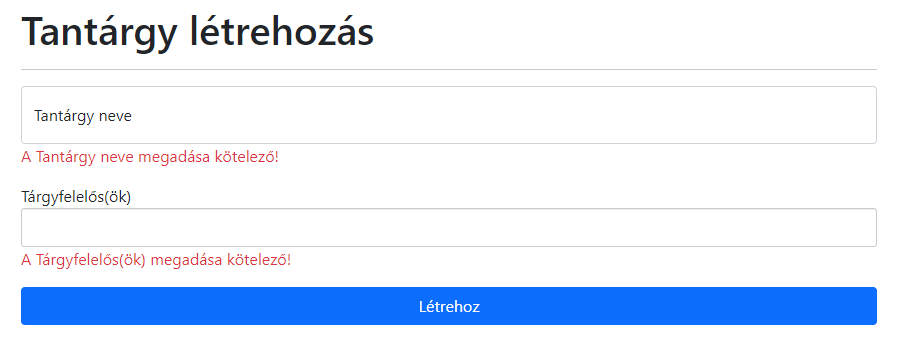
\includegraphics[width=0.8\linewidth]{userguide/admin-create-subject-error}
        \label{subfig:admin-create-subject-error}}
	\caption{Tantárgy létrehozás}
	\label{fig:admin-create-subject}
\end{figure}
\subsubsection{Felhasználó létrehozása}
Felhasználót létrehozni a ``Felhasználó létrehozás'' linkre kattintva tudjuk megtenni, ami továbbnavigál minket egy űrlapra, ahol az új felhasználónak az adatait tudjuk megadni (\ref{subfig:admin-create-user} ábra). Ha az adatok validálása sikeres, akkor a felhasználó elkészült és visszanavigálódunk a kezdőoldalra, ha nem volt sikeres, akkor a rendszer ezt hibaüzenetekkel jelzi nekünk (\ref{subfig:admin-create-user-error} ábra).
\begin{figure}[H]
	\centering
	\subfigure[Űrlap]{
		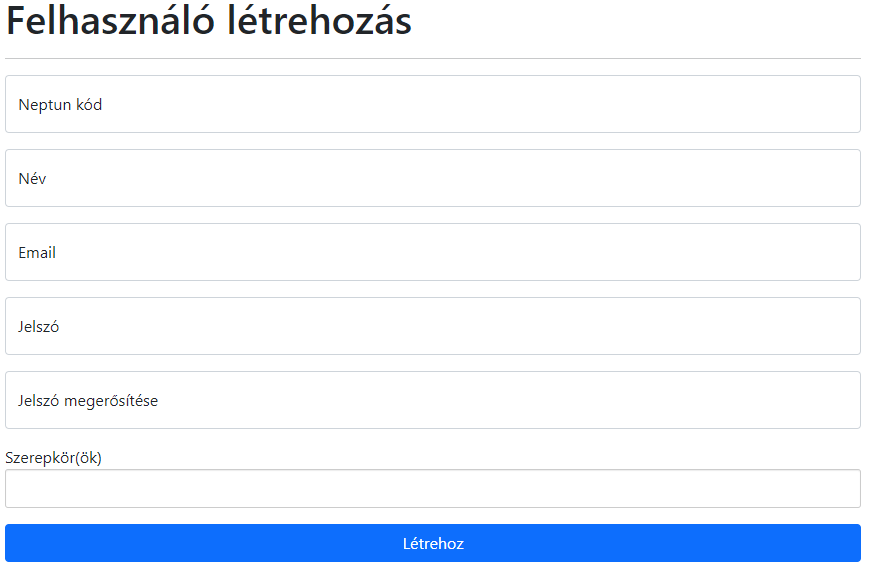
\includegraphics[width=0.7\linewidth]{userguide/admin-create-user-form}
        \label{subfig:admin-create-user}}
	\hspace{5pt}
	\subfigure[Adatok validálása]{
		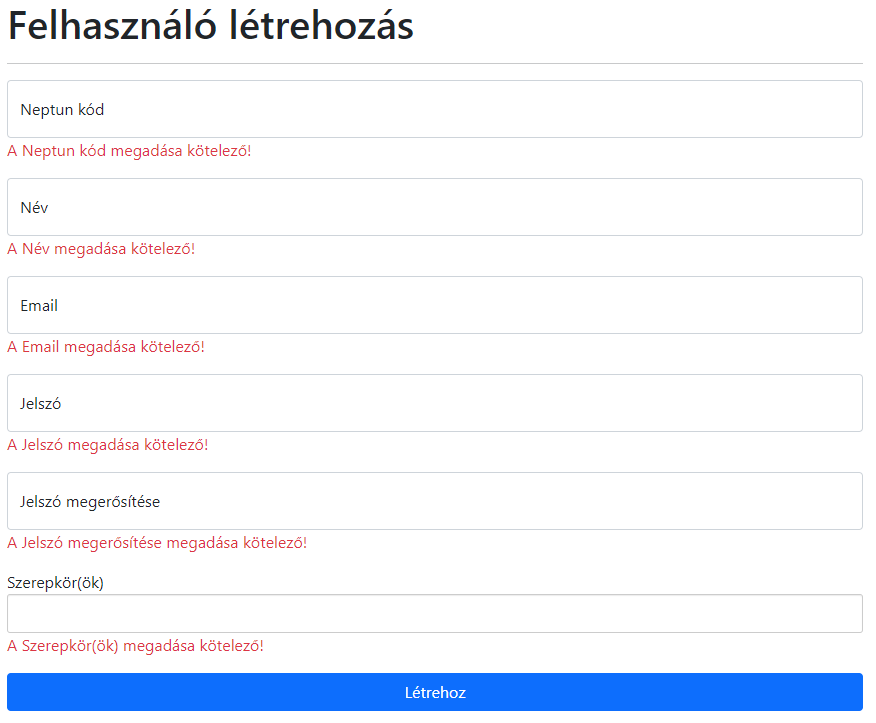
\includegraphics[width=0.85\linewidth]{userguide/admin-create-user-error}
        \label{subfig:admin-create-user-error}}
	\caption{Felhasználó létrehozás}
	\label{fig:admin-create-user}
\end{figure}
\subsection{Tárgyfelelős}\label{step:teacher-role}
Ha tárgyfelelősként jelentkezünk be a rendszerbe, akkor az alábbi kezdőoldal fogad minket (\ref{fig:teacher-home} ábra).
A kezdőoldalon egy táblázat található, amiben látjuk azokat a tantárgyakat, és a tantárgyakhoz tartozó csoportokat, amelyeknek a felelősei vagyunk.
A tárgyfelelős a következő funkciókat használhatja:
\begin{compactitem}
    \item \hyperref[step:teacher-create-course]{Csoport létrehozása egy tantárgyhoz}
    \item \hyperref[step:teacher-edit-course]{Csoport módosítása}
\end{compactitem}
\begin{figure}[H]
	\centering
	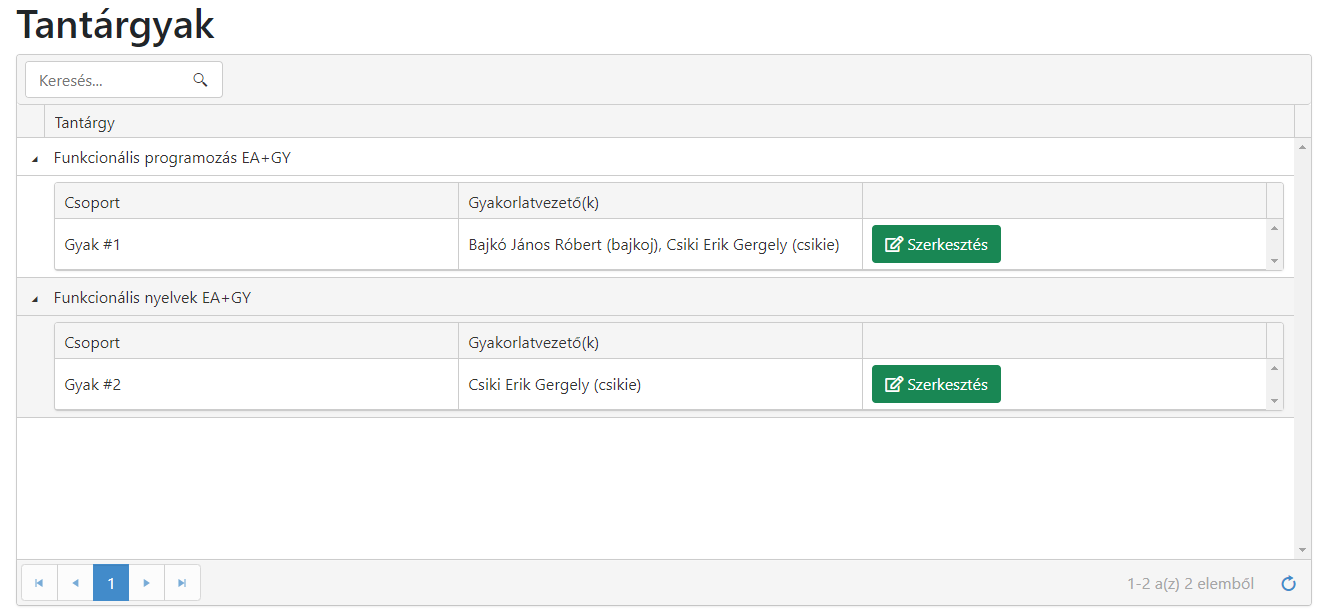
\includegraphics[width=1.0\textwidth]{userguide/teacher-home}
	\caption{Tárgyfelelős kezdőoldala}
	\label{fig:teacher-home}
\end{figure}
\subsubsection{Csoport létrehozása}
\label{step:teacher-create-course}
A menüsoron a ``Csoport létrehozás'' linkre kattintva a rendszer átirányít minket egy űrlapra, ahol létre tudunk hozni egy csoportot (\ref{fig:teacher-create-course} ábra). Az adatokat a rendszer validálja, és az esetleges hibákat jelzi számunkra.
\begin{figure}[H]
	\centering
	\subfigure[Űrlap]{
		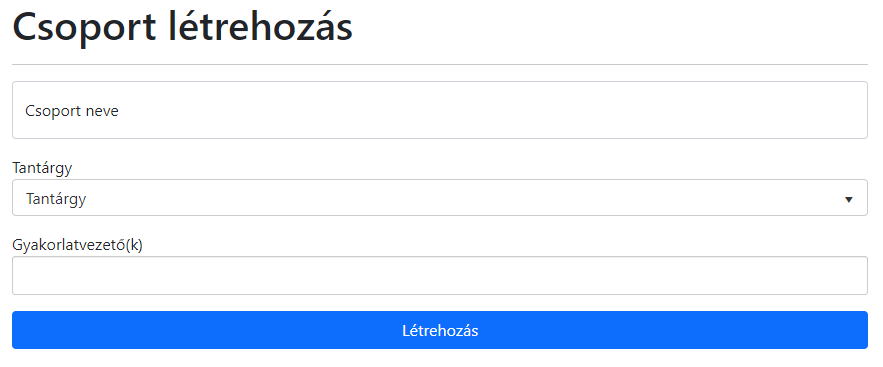
\includegraphics[width=0.75\linewidth]{userguide/teacher-create-course-form}
        \label{subfig:teacher-create-course-form}}
	\hspace{5pt}
	\subfigure[Adatok validálása]{
		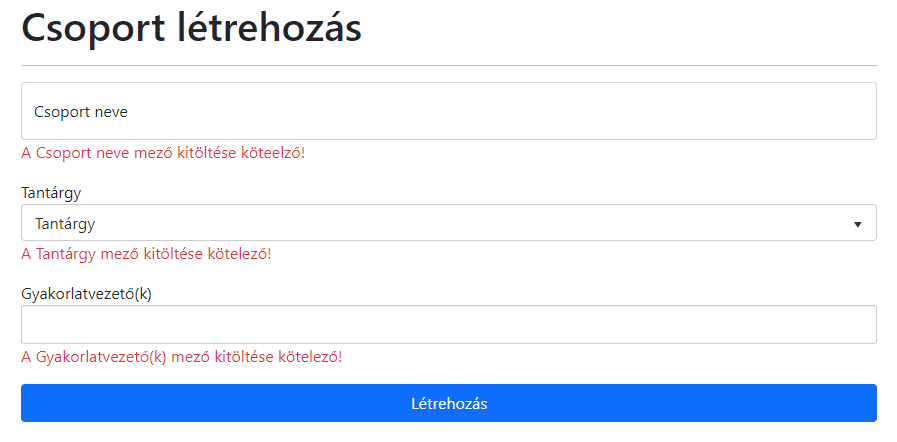
\includegraphics[width=0.75\linewidth]{userguide/teacher-create-course-error}
        \label{subfig:teacher-create-course-error}}
	\caption{Csoport létrehozás}
	\label{fig:teacher-create-course}
\end{figure}
\subsubsection{Csoport módosítása}
\label{step:teacher-edit-course}
Csoportokat szerkeszteni a kezdőoldalon található táblázat segítségével tudunk. A táblázatban lenyitható minden kilistázott tantárgy. Itt találjuk a tantárgyakhoz már létrehozott csoportokat. Minden tantárgy mellett találunk egy ``Szerkesztés'' gombot, melyre kattintva elérhetővé válik a csoport szerkesztése. Az adatok validálásra kerülnek, az esetleges hibákat a rendszer jelzi számunkra (\ref{fig:teacher-edit-course} ábra).
\begin{figure}[H]
	\centering
	\subfigure[Űrlap]{
		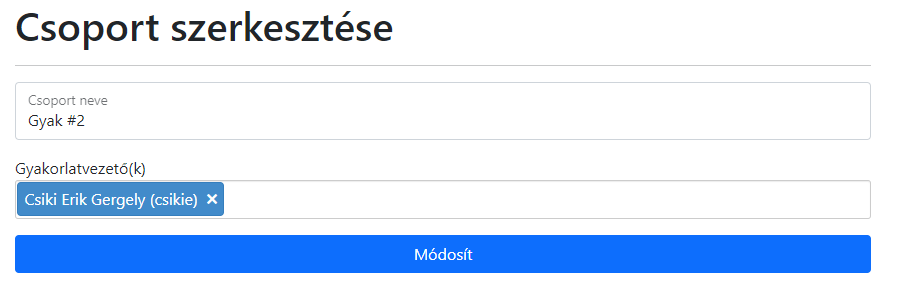
\includegraphics[width=0.75\linewidth]{userguide/teacher-edit-course-form}
        \label{subfig:teacher-edit-course-form}}
	\hspace{5pt}
	\subfigure[Adatok validálása]{
		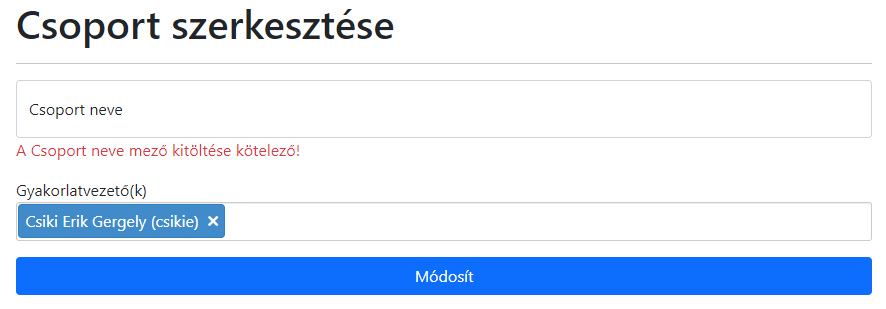
\includegraphics[width=0.75\linewidth]{userguide/teacher-edit-course-error}
        \label{subfig:teacher-edit-course-error}}
	\caption{Csoport módosítása}
	\label{fig:teacher-edit-course}
\end{figure}
\subsection{Gyakorlatvezető}\label{step:instructor-role}
Gyakorlatvezetőként bejelentkezve a rendszerbe a \ref{fig:instructor-home} ábrán látható kezdőoldal fogad minket. Az oldalon az ``Értékelendő beadandók'' cím alatt, a hozzánk rendelt csoportok hallgatóit láthatjuk egy-egy táblázatban, ahol láthatjuk, hogy egy hallgató az adott feladatra adott-e be megoldást. A ``Hallgatói várólista'' cím alatt szintén egy táblázatot találunk (\ref{subfig:instructor-table2} ábra), ahol tantárgyanként csoportosítva a következő információkat olvashatjuk le:
\begin{compactitem}
    \item Hallgató neve
	\item Hallgató neptun kódja
	\item Csoport neve
\end{compactitem}
\begin{figure}[H]
	\centering
	\subfigure[Értékelendő beadandók]{
		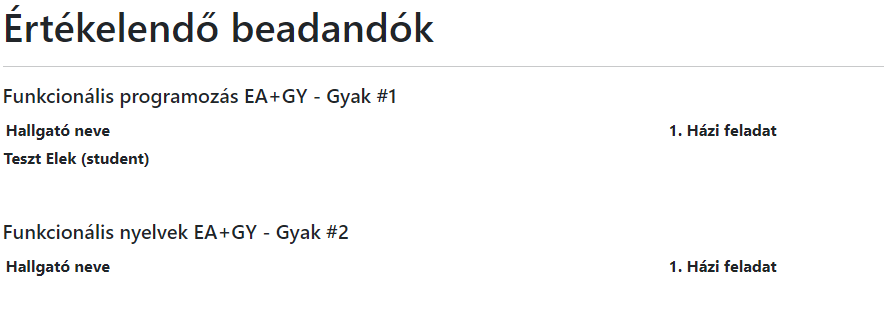
\includegraphics[width=0.75\linewidth]{userguide/instructor-table1}
        \label{subfig:instructor-table1}}
	\hspace{5pt}
	\subfigure[Hallgatói várólista]{
		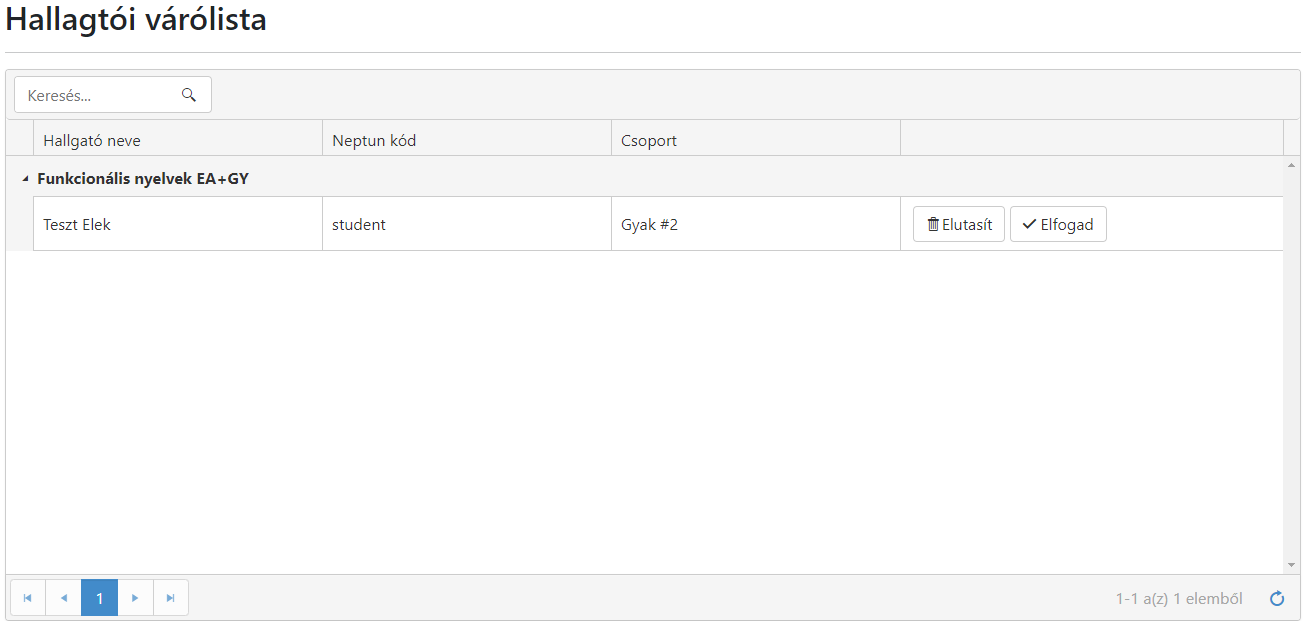
\includegraphics[width=1\linewidth]{userguide/instructor-table2}
        \label{subfig:instructor-table2}}
	\caption{Gyakorlatvezető kezdőoldala}
	\label{fig:instructor-home}
\end{figure}
A gyakorlatvezető az alábbi funkciókat éri el:
\begin{compactitem}
    \item \hyperref[step:instructor-create-assignment]{Feladat kiírása}
	\item \hyperref[step:instructor-pending]{Jelentkezések bírálata}
	\item \hyperref[step:instructor-eval]{Beadott munka értékelése}
\end{compactitem}
\subsubsection{Feladat kiírása}
\label{step:instructor-create-assignment}
Feladatot kiírni a ``Feladat létrehozása'' menüpont alatt tudunk, ahol egy űrlapot találunk (\ref{fig:instructor-create-assignment}). Ahhoz hogy létrehozzunk egy feladatot, a következő információkat szükséges megadnunk:
\begin{compactitem}
    \item A feladat neve
    \item Kezdés és befejezés dátuma
	\item Feladat leírása
	\item Mely csoporthoz legyen létrehozva\footnote{A lenyíló kiválasztó menüben lehetőségünk van több csoportot is kiválasztani}
\end{compactitem}
\begin{figure}[H]
	\centering
	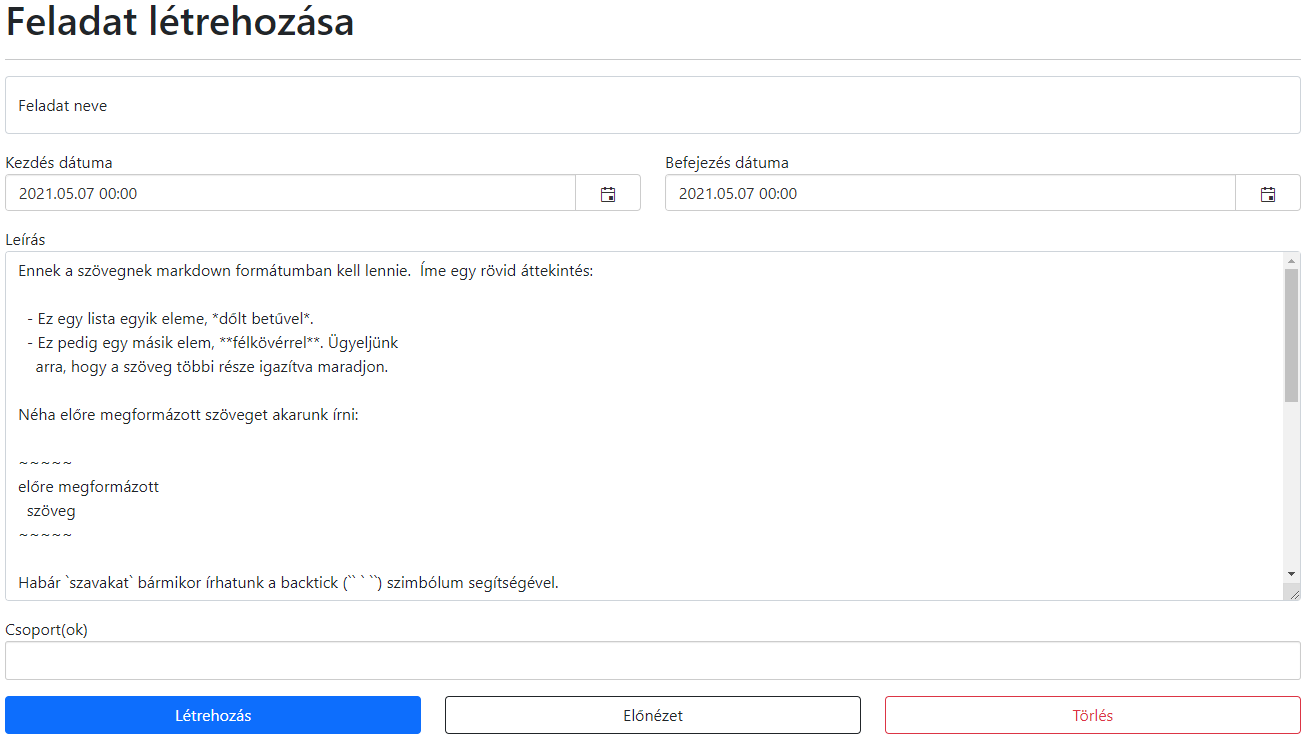
\includegraphics[width=1.0\textwidth]{userguide/instructor-create-assignment}
	\caption{Feladat létrehozás}
	\label{fig:instructor-create-assignment}
\end{figure}
A rendszer támogatja, hogy a feladatnak leírása ne csak egyszerű szöveg legyen. A szövegdobozban megadhatunk \texttt{Markdown} és \LaTeX\ kifejezéseket is. Mielőtt létrehoznánk a feladatot, meg tudjuk tekinteni, hogy a hallgató milyen formában fogja látni a kiírva a feladatot. Így le tudjuk ellenőrizni kényelmesen a feladat leírását, valamint azt is tudjuk ellenőrizni, hogy a \texttt{Markdown} és \LaTeX\ kifejezéseinket helyesen írtuk-e meg. Ha végeztünk, a ``Létrehozás'' gombbal tudjuk elküldeni a rendszernek az adatokat. Az adatokat a rendszer leellenőrzi, az esetleges hibákat jelzi számunkra (\ref{fig:instructor-create-assignment-error}).
\begin{figure}[H]
	\centering
	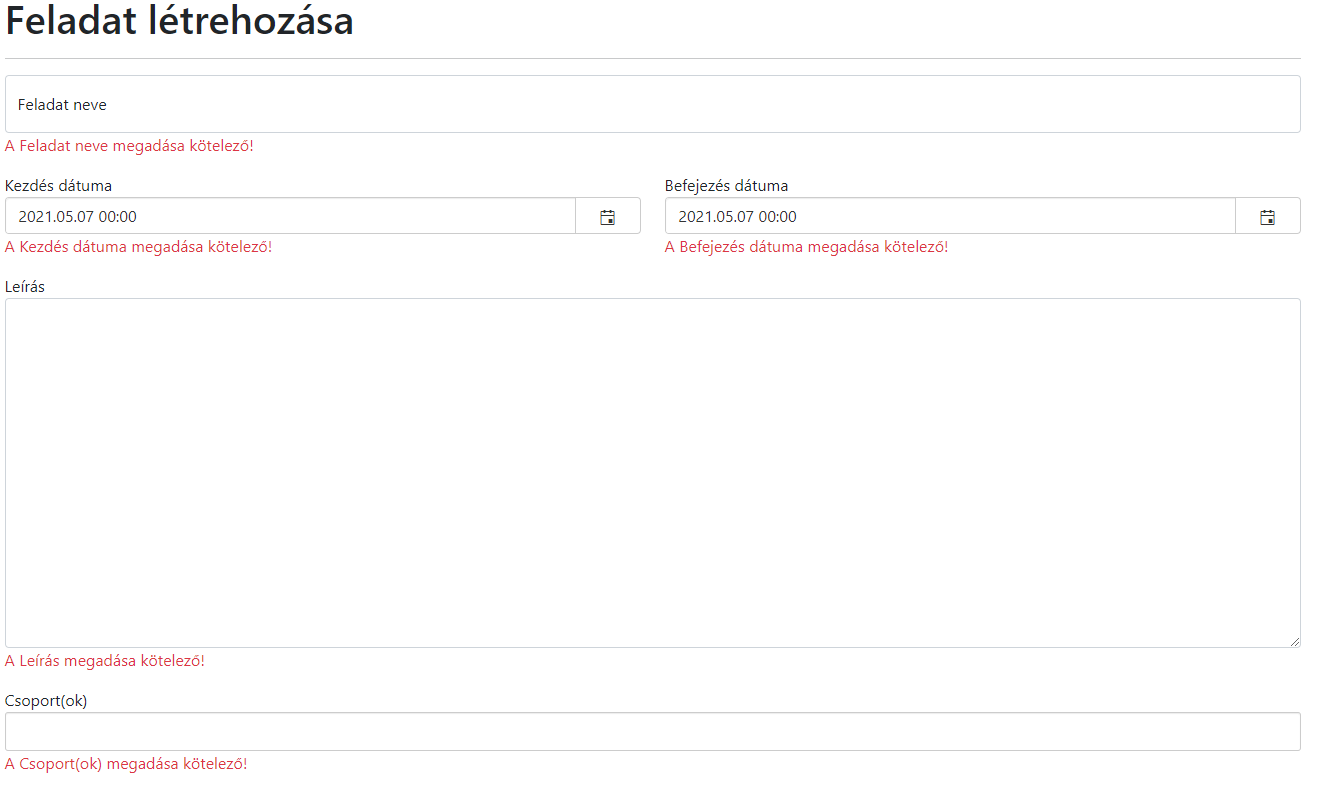
\includegraphics[width=1.0\textwidth]{userguide/instructor-create-assignment-error}
	\caption{Adatok validálása}
	\label{fig:instructor-create-assignment-error}
\end{figure}
\subsubsection{Jelentkezések bírálata}
\label{step:instructor-pending}
Egy hallgatónak a csoportba való jelentkezését a ``Hallgatói várólista'' táblázatában tudjuk megtenni (\ref{subfig:instructor-table2} ábra), az utolsó oszlopban lévő gombok segítségével. Miután elvégeztük a bírálatot, a táblázatból törlődik a jelentkezett hallgató, és az oldal frissítése után, a megfelelő táblázatban látjuk, hogy a hallgatót a rendszer felvette a jelentkezett csoportba.
\subsubsection{Beadott munka értékelése}
\label{step:instructor-eval}
Egy feladatra beadott megoldás értékeléséhez a kívánt feladat oszlopában kattintsunk a \emph{szürke négyzetre}. Ilyenkor a rendszer átirányít minket az értékelő felületre (\ref{fig:instructor-eval-assignment}). A rendszer a felületre a ``Megoldás(ok)'' alatt felsorolja a hallgatónak az összes beadott megoldását a beküldés ideje szerint csökkenően rendezve. Elég egy megoldást értékelnünk, de értékelhetjük az összeset is. Viszont a rendszer a legutolsó értékelést veszi számításba. Ezt fogja a hallgató is látni. A beadott megoldások között a kívánt sorra kattintva tudjuk kiválasztani, hogy melyik megoldást szeretnénk változtatni. Ilyenkor a ``Beadott megoldás'' alatt látjuk, mi a hallgatónak a beadott megoldása. Az értékelésünket az oldal alján található űrlapon tudjuk megtenni. Az értékelés után a rendszer a kezdőoldalra navigál minket. Az értékelt feladatnál a \emph{szürke négyzet} egy \emph{körben lévő pipára} cserélődik.
\begin{figure}[H]
	\centering
	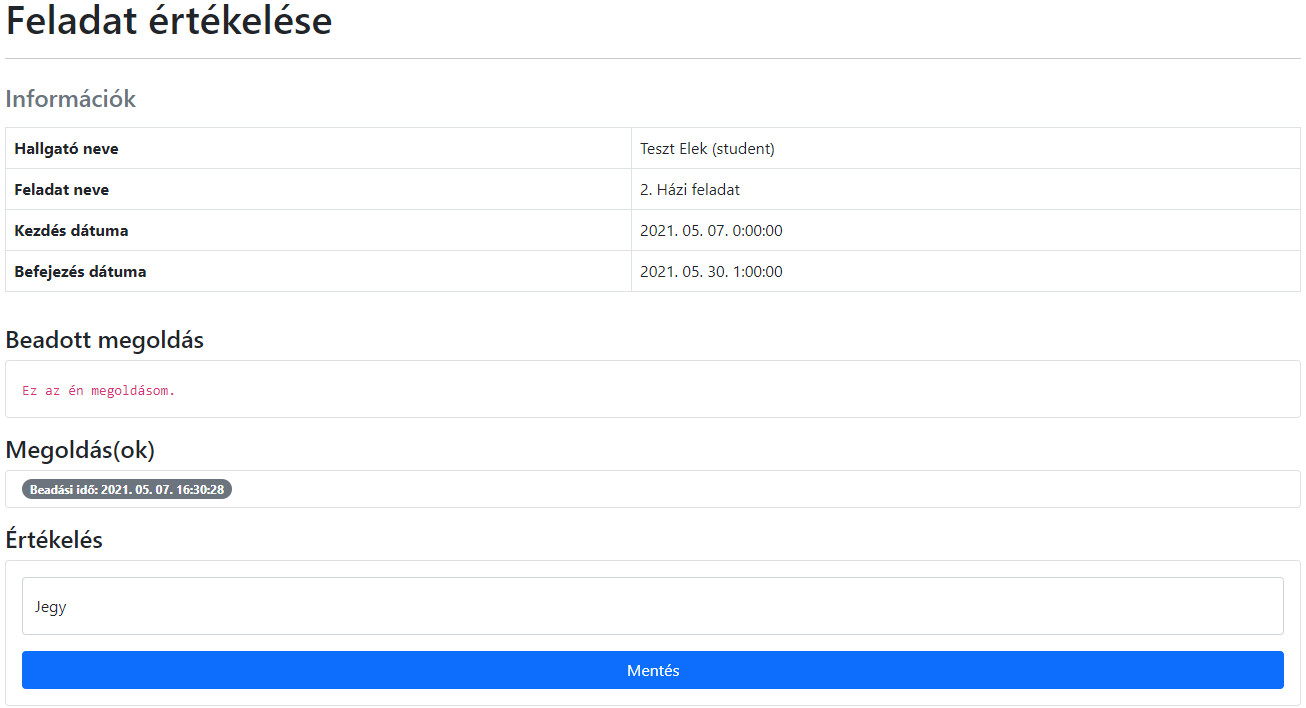
\includegraphics[width=1.0\textwidth]{userguide/instructor-eval-assignment}
	\caption{Feladat értékelése}
	\label{fig:instructor-eval-assignment}
\end{figure}
\subsection{Hallgató}
\label{step:student-role}
Hallgatóként bejelentkezve a \ref{fig:student-home} ábrán látható kezdőoldal fogad minket. A ``Feladatok'' cím alatti táblázatban a hallgató számára listázásra kerül az összes olyan csoportja, ahova elfogadták a jelentkezését. A táblázatban csoportokra lebontva jelennek meg a hallgató számára a kiírt feladatok. A táblázatban egy feladatról a következő információkat láthatjuk: neve, határideje, kapott értékelés.
\begin{figure}[H]
	\centering
	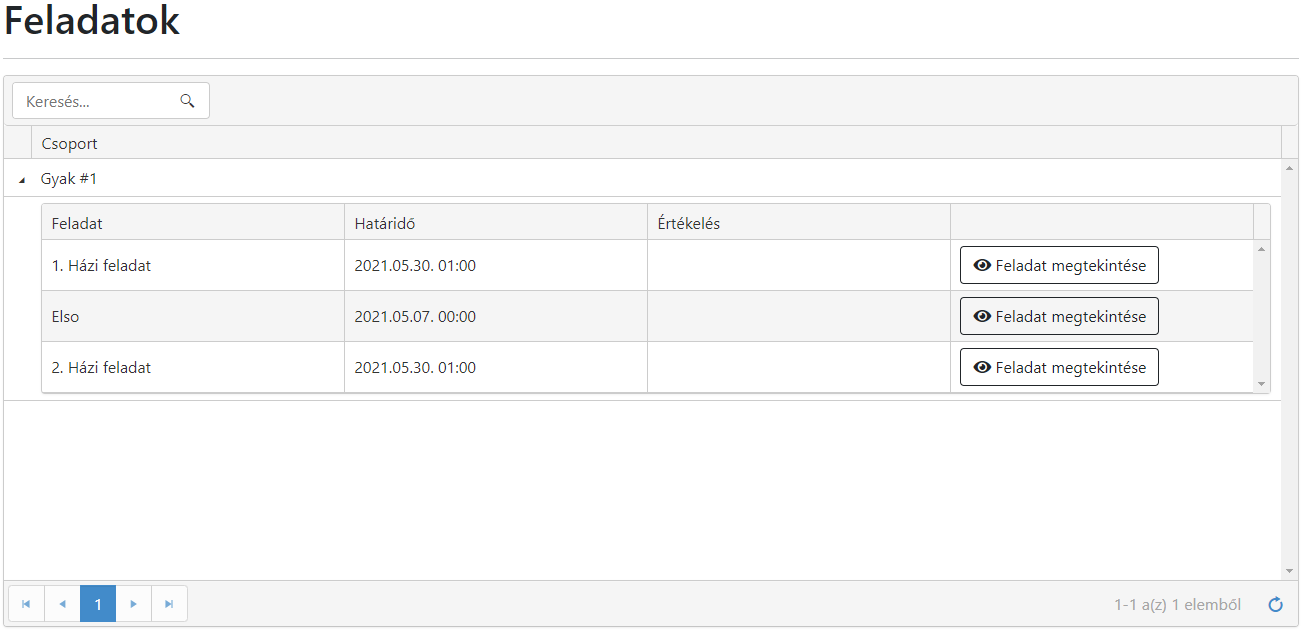
\includegraphics[width=1.0\textwidth]{userguide/student-home}
	\caption{Hallgató kezdőoldala}
	\label{fig:student-home}
\end{figure}
A hallgató az alábbi funkciókat használhatja:
\begin{compactitem}
    \item \hyperref[step:student-course-reg]{Csoportba jelentkezés}
	\item \hyperref[step:student-solution]{Megoldás beadása}
\end{compactitem}
\subsubsection{Csoportba jelentkezés}
\label{step:student-course-reg}
Csoportba jelentkezni a ``Csoport jelentkezés'' menüpontra kattintva tudunk. A rendszer egy űrlapot biztosít számunkra (\ref{fig:student-course-reg} ábra), ahol listázásra kerülnek a rendszerben található csoportok, amelyekre még nem jelentkeztünk. A rendszer lehetőséget biztosít számunkra, hogy akár egyszerre több csoportra is leadjuk a jelentkezésünket. Jelentkezésünket a ``Jelentkezés'' gombbal tudjuk továbbítani a rendszer számára. Az űrlap validálásra kerül, hogy üresen ne tudjuk beküldeni azt. Sikeres jelentkezés esetén a rendszer a kezdőoldalra navigál minket.
\begin{figure}[H]
	\centering
	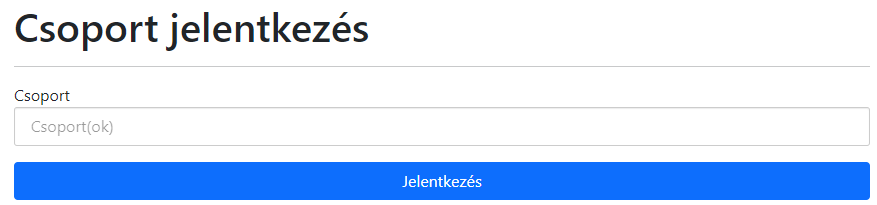
\includegraphics[width=1.0\textwidth]{userguide/student-course-reg}
	\caption{Csoportba jelentkezése}
	\label{fig:student-course-reg}
\end{figure}
\subsubsection{Megoldás beadása}
\label{step:student-solution}
Megoldás beküldéséhez válasszuk ki a kívánt feladatot, amire megoldást szeretnénk beküldeni, majd kattintsunk a ``Feladat megtekintése'' gombra. Ekkor a rendszer egy új ablakban megnyitja a feladatot (\ref{fig:student-submit-sol} ábra). Az oldalon a következő információkat látjuk:
\begin{compactitem}
    \item Határidő visszaszámláló
    \item Feladat neve, leírása
    \item Beküldött megoldások
    \item Űrlap a megoldás beküldéséhez
\end{compactitem}
\begin{figure}[H]
	\centering
	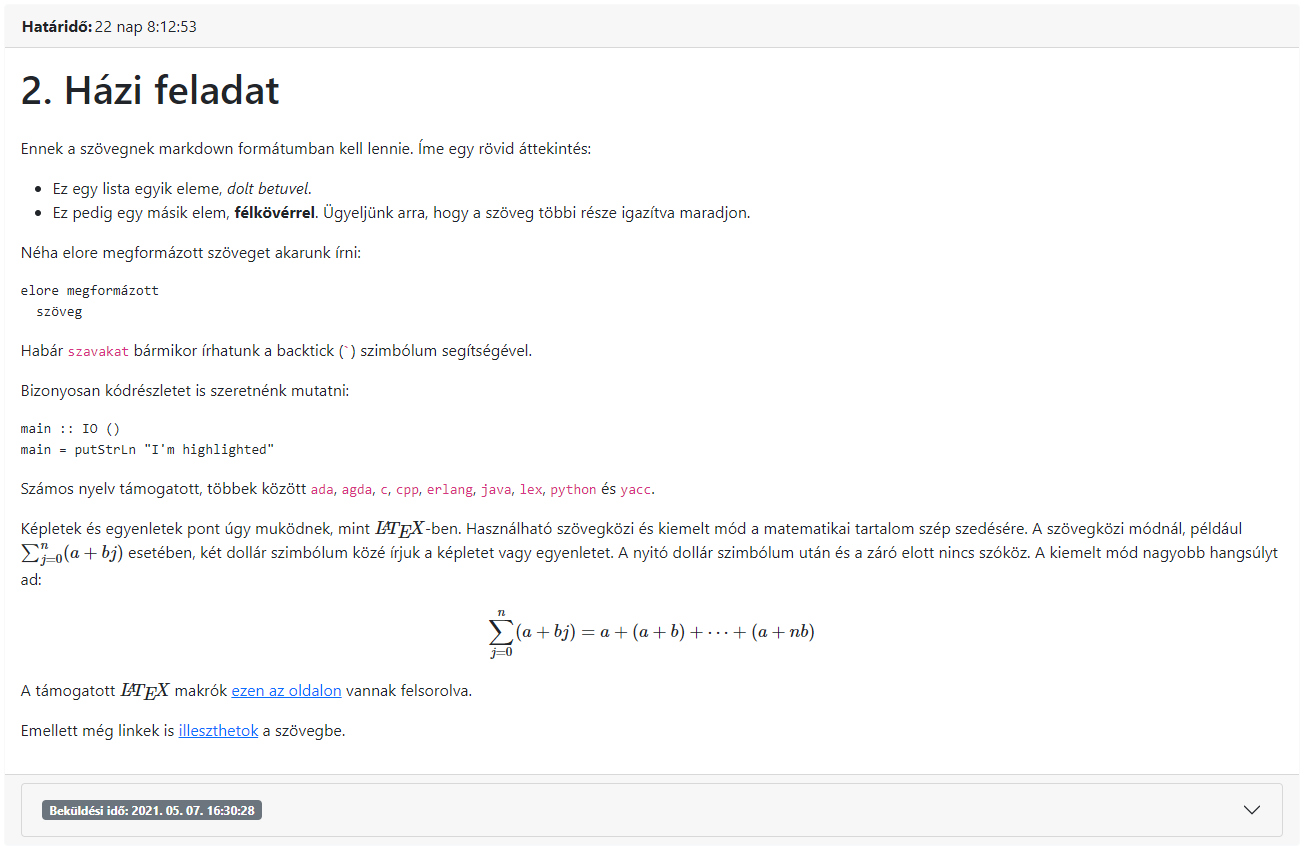
\includegraphics[width=1.0\textwidth]{userguide/student-submit-sol}
	\caption{Feladat megtekintése}
	\label{fig:student-submit-sol}
\end{figure}
\subsection{Mindenki számára elérhető oldalak}
\label{step:mindenkinek-elerheto-oldal}
A rendszerben jelenleg három olyan oldal található, amelyet minden szerepkörben elérhetünk. Az egyik oldal a felhasználónk adatainak megtekintésére szolgál. Ezt a funkciót a menüsoron a nevünkre kattintva tudjuk elérni. Ezen a felületen (\ref{fig:profile} ábra) a következőket tekinthetjük meg a ``Személyes adatok'' cím alatt: név, neptun kód, e-mail cím és a felhasználónkhoz rendelt szerepkörök. Ezen felületen továbbá be tudjuk állítani, hogy a rendszer milyen lokalizációval működjön (magyar és angol). Ezt a megfelelő gombra kattintva tudjuk változtatni.
\begin{figure}[H]
	\centering
	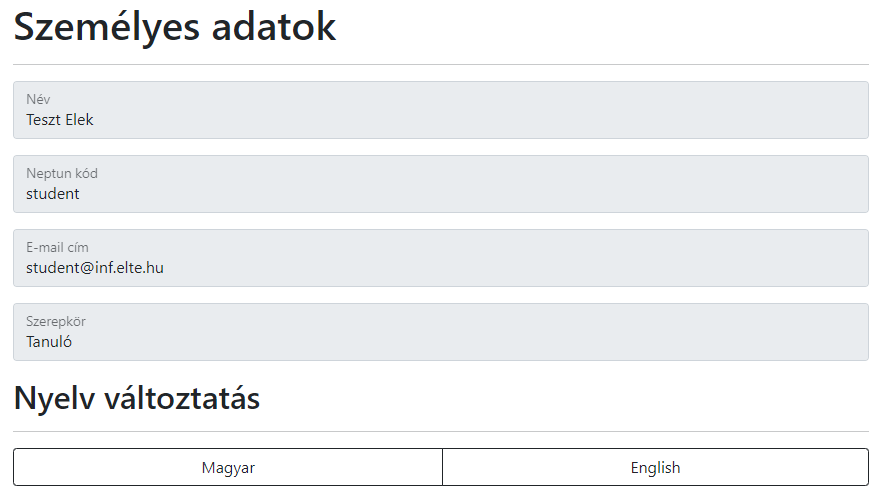
\includegraphics[width=0.8\textwidth]{userguide/profil}
	\caption{Profil oldal}
	\label{fig:profile}
\end{figure}
A másik két oldal az esetleges nem várt hibákról tájékoztat minket. Ezen hibák két kategóriába oszthatók: jogosulatlan kérés a rendszer felé, egyéb nem várt hiba. Jogosulatlan kérés akkor lép fel, ha megpróbálunk a szerepkörünkhöz nem tartozó funkciót elérni a rendszerben. Például: csak hallgatói szerepkörrel rendelkező felhasználóval vagyunk bejelentkezve a rendszerbe és a webcím végén a ``Student''-et lecseréljük ``Admin''-ra. Ezzel olyan kérést indítunk a rendszernek, hogy navigáljon minket a rendszergazdai szerepkörhöz tartozó kezdőoldalra, amihez nincs jogosultságunk, ezért a rendszer megtagadja a hozzáférést a kért oldalhoz. Ilyenkor a rendszer az alábbi \ref{fig:access-denied} ábrán látható oldalra navigál minket, ahonnan lehetőségünk van visszatérni a szerepkörünkhöz tartozó kezdőoldalra.
\begin{figure}[H]
	\centering
	
\includegraphics[width=1.0\textwidth]{userguide/access-denied}
	\caption{Jogosulatlan kérés}
	\label{fig:access-denied}
\end{figure}
Egyéb nem várt hiba lehet például, hogy a rendszer nem tud csatlakozni a hozzá tartozó adatbázishoz. Ilyenkor az alábbi \ref{fig:errors} ábrán látható oldalra navigál minket.
\begin{figure}[H]
	\centering
	
\includegraphics[width=1.0\textwidth]{userguide/errors}
	\caption{Egyéb nem várt hiba}
	\label{fig:errors}
\end{figure}
\cleardoublepage

\chapter{Fejlesztői dokumentáció} % Developer guide
\label{ch:impl}

Lorem ipsum dolor sit amet, consectetur adipiscing elit. Duis nibh leo, dapibus in elementum nec, aliquet id sem. Suspendisse potenti. Nullam sit amet consectetur nibh. Donec scelerisque varius turpis at tincidunt.


\section{Tételek, definíciók, megjegyzések} % Theorem-like items

\begin{definition}
Mauris tristique sollicitudin ultrices. Etiam tristique quam sit amet metus dictum imperdiet. Nunc id lorem sed nisl pulvinar aliquet vitae quis arcu. Morbi iaculis eleifend porttitor.
\end{definition}

Maecenas rutrum eros sem, pharetra interdum nulla porttitor sit amet. In vitae viverra ante. Maecenas sit amet placerat orci, sed tincidunt velit. Vivamus mattis, enim vel suscipit elementum, quam odio venenatis elit, et mollis nulla nunc a risus. Praesent purus magna, tristique sed lacus sit amet, convallis malesuada magna. Phasellus faucibus varius purus, nec tristique enim porta vitae.

\begin{theorem}
Nulla finibus ante vel arcu tincidunt, ut consectetur ligula finibus. Mauris mollis lectus sed ipsum bibendum, ac ultrices erat dictum. Suspendisse faucibus euismod lacinia. Etiam vel odio ante.
\end{theorem}
\begin{proof}
Etiam pulvinar nibh quis massa auctor congue. Pellentesque quis odio vitae sapien molestie vestibulum sit amet et quam. Pellentesque vel dui eget enim hendrerit finibus at sit amet libero. Quisque sollicitudin ultrices enim, nec porta magna imperdiet vitae. Cras condimentum nunc dui.
\end{proof}

Donec dapibus sodales ante, at scelerisque nunc laoreet sit amet. Mauris porttitor tincidunt neque, vel ullamcorper neque pulvinar et. Integer eu lorem euismod, faucibus lectus sed, accumsan felis. 

\begin{remark}
Nunc ornare mi at augue vulputate, eu venenatis magna mollis. Nunc sed posuere dui, et varius nulla. Sed mollis nibh augue, eget scelerisque eros ornare nec. Praesent porta, metus eget eleifend consequat, eros ligula eleifend ex, a pellentesque mi est vitae urna. Vivamus turpis nunc, iaculis non leo eget, mattis vulputate tellus.
\end{remark}

Fusce in aliquet neque, in pretium sem. Donec tincidunt tellus id lectus pretium fringilla. Nunc faucibus, erat pretium tempus tempor, tortor mi fringilla neque, ac congue ex dui vitae mauris. Donec pretium et quam a cursus.

\begin{note}
Aliquam vehicula luctus mi a pretium. Nulla quam neque, maximus nec velit in, aliquam mollis tortor. Aliquam erat volutpat. Curabitur vitae laoreet turpis. Integer id diam ligula.
\end{note}

Ut sollicitudin tempus urna et mollis. Aliquam et aliquam turpis, sed fermentum mauris. Nulla eget ex diam. Donec eget tellus pharetra, semper neque eget, rutrum diam.

\subsection{Egyenletek, matematika} % Equations, formulas

Duis suscipit ipsum nec urna blandit, $2 + 2 = 4$ pellentesque vehicula quam fringilla. Vivamus euismod, lectus sit amet euismod viverra, dolor metus consequat sapien, ut hendrerit nisl nulla id nisi. Nam in leo eu quam sollicitudin semper a quis velit.

$$a^2 + b^2 = c^2$$

Phasellus mollis, elit sed convallis feugiat, dolor quam dapibus nibh, suscipit consectetur lacus risus quis sem. Vivamus scelerisque porta odio, vitae euismod dolor accumsan ut.

In mathematica, identitatem Euleri (equation est scriptor vti etiam notum) sit aequalitatem Equation~\ref{eq:euler}:
\begin{equation}\label{eq:euler}
e^{i \times \pi} + 1 = 0
\end{equation}


\section{Forráskódok} % Source code samples

Nulla sodales purus id mi consequat, eu venenatis odio pharetra. Cras a arcu quam. Suspendisse augue risus, pulvinar a turpis et, commodo aliquet turpis. Nulla aliquam scelerisque mi eget pharetra. Mauris sed posuere elit, ac lobortis metus. Proin lacinia sit amet diam sed auctor. Nam viverra orci id sapien sollicitudin, a aliquam lacus suscipit. Quisque ac tincidunt leo Code~\ref{src:cpp} and \ref{src:csharp}:

\lstset{caption={Hello World in C++}, label=src:cpp}
\begin{lstlisting}[language={C++}]
#include <stdio>

int main() 
{
	int c;
	std::cout << "Hello World!" << std::endl;

	std::cout << "Press any key to exit." << std::endl;
	std::cin >> c;
	
	return 0;
}
\end{lstlisting}

\lstset{caption={Hello World in C\#}, label=src:csharp}
\begin{lstlisting}[language={[Sharp]C}]
using System;
namespace HelloWorld
{
	class Hello 
	{
		static void Main() 
		{
			Console.WriteLine("Hello World!");
			
			Console.WriteLine("Press any key to exit.");
			Console.ReadKey();
		}
	}
}
\end{lstlisting}

\subsection{Algoritmusok} % Algorithms

A general Interval Branch and Bound algorithm is shown in Algorithm~\ref{alg:ibb}. One of the following selection rules is applied in Step \ref{step:selrule}.\\
Példa forrása: \href{https://www.inf.u-szeged.hu/actacybernetica/}{Acta Cybernetica (ez egy link)}.

\begin{algorithm}[H]
\caption{A general interval B\&B algorithm} 
\label{alg:ibb} 
\textbf{\underline{Funct}} IBB($S,f$)
\begin{algorithmic}[1] % sorszámok megjelenítése minden n. sor előtt, most n = 1
\STATE Set the working list ${\cal L}_W$ := $\{S\}$ and the final list ${\cal L}_Q$ := $\{\}$     
\WHILE{( ${\cal L}_W \neq \emptyset$ )} \label{alg:igoend}
	\STATE  Select an interval $X$ from ${\cal L}_W$ \label{step:selrule}\COMMENT{Selection rule}  
	\STATE Compute $lbf(X)$ \COMMENT{Bounding rule}		  
	\IF[Elimination rule]{$X$ cannot be eliminated}
		\STATE Divide $X$ into $X^j,\ j=1,\dots, p$, subintervals   \COMMENT{Division rule}
		\FOR{$j=1,\ldots,p$}
			\IF[Termination rule]{$X^j$ satisfies the termination criterion}
				\STATE Store $X^j$ in ${\cal L}_W$ 
			\ELSE
				\STATE Store $X^j$ in ${\cal L}_W$ 
			\ENDIF
		\ENDFOR  
	\ENDIF
\ENDWHILE
\STATE \textbf{return} ${\cal L}_Q$
\end{algorithmic}
\end{algorithm}

\cleardoublepage

\chapter{Összegzés} % Conclusion
\label{ch:sum}

Lorem ipsum dolor sit amet, consectetur adipiscing elit. In eu egestas mauris. Quisque nisl elit, varius in erat eu, dictum commodo lorem. Sed commodo libero et sem laoreet consectetur. Fusce ligula arcu, vestibulum et sodales vel, venenatis at velit. Aliquam erat volutpat. Proin condimentum accumsan velit id hendrerit. Cras egestas arcu quis felis placerat, ut sodales velit malesuada. Maecenas et turpis eu turpis placerat euismod. Maecenas a urna viverra, scelerisque nibh ut, malesuada ex.

Aliquam suscipit dignissim tempor. Praesent tortor libero, feugiat et tellus porttitor, malesuada eleifend felis. Orci varius natoque penatibus et magnis dis parturient montes, nascetur ridiculus mus. Nullam eleifend imperdiet lorem, sit amet imperdiet metus pellentesque vitae. Donec nec ligula urna. Aliquam bibendum tempor diam, sed lacinia eros dapibus id. Donec sed vehicula turpis. Aliquam hendrerit sed nulla vitae convallis. Etiam libero quam, pharetra ac est nec, sodales placerat augue. Praesent eu consequat purus.

\cleardoublepage

% Függelékek (opcionális) - hosszabb részletező táblázatok, sok és/vagy nagy kép esetén hasznos
% Appendices (optional) - useful for detailed information in long tables, many and/or large figures, etc.
\appendix
\chapter{Szimulációs eredmények} % Simulation results
\label{appx:simulation}

Lorem ipsum dolor sit amet, consectetur adipiscing elit. Pellentesque facilisis in nibh auctor molestie. Donec porta tortor mauris. Cras in lacus in purus ultricies blandit. Proin dolor erat, pulvinar posuere orci ac, eleifend ultrices libero. Donec elementum et elit a ullamcorper. Nunc tincidunt, lorem et consectetur tincidunt, ante sapien scelerisque neque, eu bibendum felis augue non est. Maecenas nibh arcu, ultrices et libero id, egestas tempus mauris. Etiam iaculis dui nec augue venenatis, fermentum posuere justo congue. Nullam sit amet porttitor sem, at porttitor augue. Proin bibendum justo at ornare efficitur. Donec tempor turpis ligula, vitae viverra felis finibus eu. Curabitur sed libero ac urna condimentum gravida. Donec tincidunt neque sit amet neque luctus auctor vel eget tortor. Integer dignissim, urna ut lobortis volutpat, justo nunc convallis diam, sit amet vulputate erat eros eu velit. Mauris porttitor dictum ante, commodo facilisis ex suscipit sed.

Sed egestas dapibus nisl, vitae fringilla justo. Donec eget condimentum lectus, molestie mattis nunc. Nulla ac faucibus dui. Nullam a congue erat. Ut accumsan sed sapien quis porttitor. Ut pellentesque, est ac posuere pulvinar, tortor mauris fermentum nulla, sit amet fringilla sapien sapien quis velit. Integer accumsan placerat lorem, eu aliquam urna consectetur eget. In ligula orci, dignissim sed consequat ac, porta at metus. Phasellus ipsum tellus, molestie ut lacus tempus, rutrum convallis elit. Suspendisse arcu orci, luctus vitae ultricies quis, bibendum sed elit. Vivamus at sem maximus leo placerat gravida semper vel mi. Etiam hendrerit sed massa ut lacinia. Morbi varius libero odio, sit amet auctor nunc interdum sit amet.

Aenean non mauris accumsan, rutrum nisi non, porttitor enim. Maecenas vel tortor ex. Proin vulputate tellus luctus egestas fermentum. In nec lobortis risus, sit amet tincidunt purus. Nam id turpis venenatis, vehicula nisl sed, ultricies nibh. Suspendisse in libero nec nisi tempor vestibulum. Integer eu dui congue enim venenatis lobortis. Donec sed elementum nunc. Nulla facilisi. Maecenas cursus id lorem et finibus. Sed fermentum molestie erat, nec tempor lorem facilisis cursus. In vel nulla id orci fringilla facilisis. Cras non bibendum odio, ac vestibulum ex. Donec turpis urna, tincidunt ut mi eu, finibus facilisis lorem. Praesent posuere nisl nec dui accumsan, sed interdum odio malesuada.
\cleardoublepage

% Irodalomjegyzék (kötelező)
% Bibliography (mandatory)
\addcontentsline{toc}{chapter}{\biblabel}
\printbibliography[title=\biblabel]
\cleardoublepage

% Ábrajegyzék (opcionális) - 3-5 ábra fölött érdemes
% List of figures (optional) - useful over 3-5 figures
\addcontentsline{toc}{chapter}{\lstfigurelabel}
\listoffigures
\cleardoublepage

% Táblázatjegyzék (opcionális) - 3-5 táblázat fölött érdemes
% List of tables (optional) - useful over 3-5 tables
\addcontentsline{toc}{chapter}{\lsttablelabel}
\listoftables
\cleardoublepage

% Forráskódjegyzék (opcionális) - 3-5 kódpélda fölött érdemes
% List of codes (optional) - useful over 3-5 code samples
\addcontentsline{toc}{chapter}{\lstcodelabel}
\lstlistoflistings
\cleardoublepage

% Jelölésjegyzék (opcionális)
% List of symbols (optional)
%\printnomenclature

\end{document}
